\documentclass{beamer}
\usepackage[utf8]{inputenc}
\usepackage[T1]{fontenc}
\usepackage{lipsum, lmodern}
\usepackage[scaled=.95]{helvet}% helvetica as the origin of arial
\usepackage[helvet]{sfmath}    % for the mathematical enviroments
\usepackage{graphicx}
\usepackage{multimedia}% for add a movie
\usepackage{hyperref}
\usepackage{media9} %for movie : 

% To simplify for people wiwithout knowledge on Latex
\usepackage{array}% Tableau si besoin
\usepackage{multirow}
\usepackage{rotating,tabularx}
\usepackage{hyperref} % Pour créer des liens hypertexts: \url{my_url}
\usepackage{multirow}
\usepackage{pdflscape}
\usepackage{amsmath} % Equation non numŽrotŽe et autres
\usepackage{esint} % double, triple integrals
\usepackage{amssymb}
\usepackage{amsfonts}
\usepackage{mathtools}
\usepackage{empheq}
\usepackage{array}
\usepackage{dsfont} % Ensembles C,R,N ,...
% End of package add from my last projects

\renewcommand{\familydefault}{\sfdefault}

%% ETH beamer theme
% Options: [default]
%   itemsblack/[itemsblue]: change color of bullets etc. to black/blue in itemize style environments
%   [titlesblack]/titlesblue: change color of frame titles/subtitles to black/blue
% \usetheme[itemsblack,titlesblack]{eth}
\usetheme{eth}

%% Theme uses ETH blue color by default. Can be changed to any color using this command: 
% \setbeamercolor{structure}{fg=blue}

%% Mandatory variables
\author{Jasmin Fischli, Philipp Göldlin, Julie Veya, Jonathan Burkhard}
\title{Paper presentation : UltraStereo: Efficient Learning-based Matching for Active Stereo Systems}
\date{\today}

%% Optional variables
 \supervisor{Sattler Torsten} % for one supervisor
%\supervisors{Carol Foote, Jane Smith} % for multiple supervisors
% \projecttype{Master's Thesis}

\begin{document}

\frame{\maketitle}
\begin{frame}{Table of contents}{}
	\tableofcontents
\end{frame}

%%%%%%%%%%%%%%%%%%%%%%%%%%%%%%%%%%%%%%%%%%%%%%%%%%%%%%%%%%%%%%%%%%%%%%%%%%%%
%
% Part from each person
%
%%%%%%%%%%%%%%%%%%%%%%%%%%%%%%%%%%%%%%%%%%%%%%%%%%%%%%%%%%%%%%%%%%%%%%%%%%%%
%%%%%%%%%%%%%%%%%%%%%%%%%%%%%%%%%%%%%%%%%%%%%%%%%%%%%%%%%%%%%%%%%%%%%%%%%%%%%%%%%
%
% Philipp's part
%
%%%%%%%%%%%%%%%%%%%%%%%%%%%%%%%%%%%%%%%%%%%%%%%%%%%%%%%%%%%%%%%%%%%%%%%%%%%%%%%%%
\section{State of the art methods}
\begin{frame}{Time of flight}

Varying active illumination to reconstruct a scene from multiple images
\begin{figure}
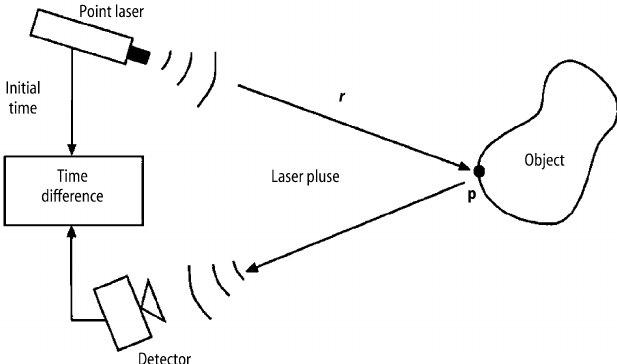
\includegraphics[scale=0.15]{pictures/polop2}
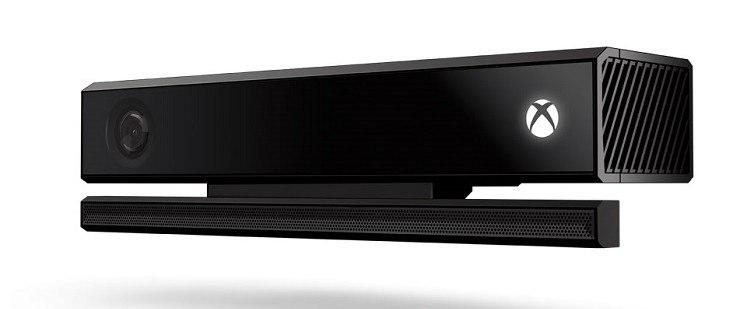
\includegraphics[scale=0.2]{pictures/polop1}
\end{figure}
Shortcomings:
\begin{itemize}
\item Low mapping rate (~30Hz)
\item Motion artifacts
\item Multipath-interference
\end{itemize}
\end{frame}


%%%%%%%%%%%%%%%%%%%%%%%%%%%%%%%%%%%%%%%
\begin{frame}{Structured Light}

Spatial patterns projected on the scene
\begin{figure}
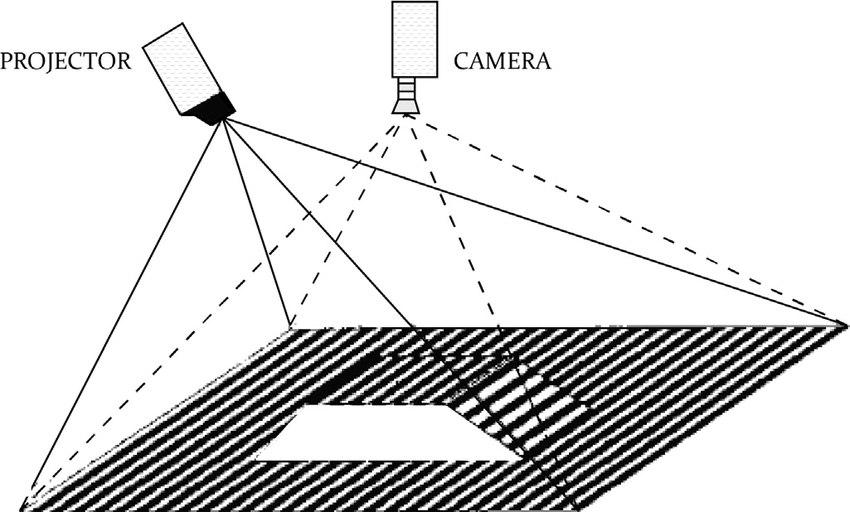
\includegraphics[scale=0.1]{pictures/polop4}
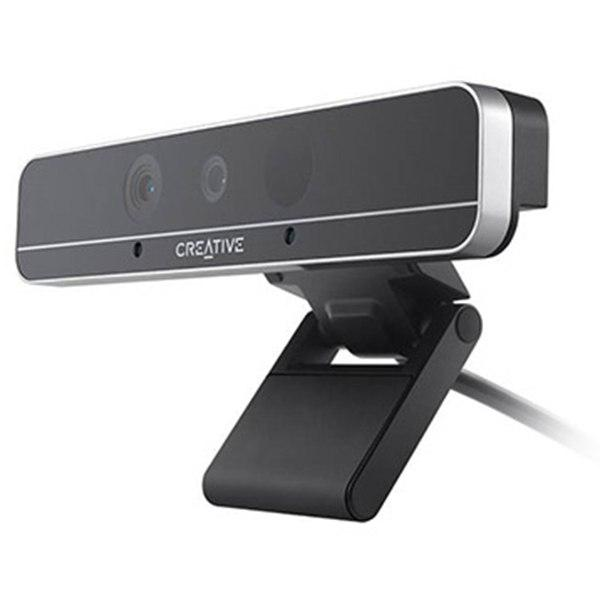
\includegraphics[scale=0.1]{pictures/polop3}
\end{figure}
Shortcomings:
\begin{itemize}
\item Robustness issues
\item Motion artifacts
\item Limited depth-range
\item Overlapping sensors cause interference
\end{itemize}
\end{frame}



%%%%%%%%%%%%%%%%%%%%%%%%%%%%%%%%%%%%%%%%

\begin{frame}{Active Stereo}

Using 2 calibrated cameras and 1 light source - solves a lot of the mentioned issues
\begin{figure}
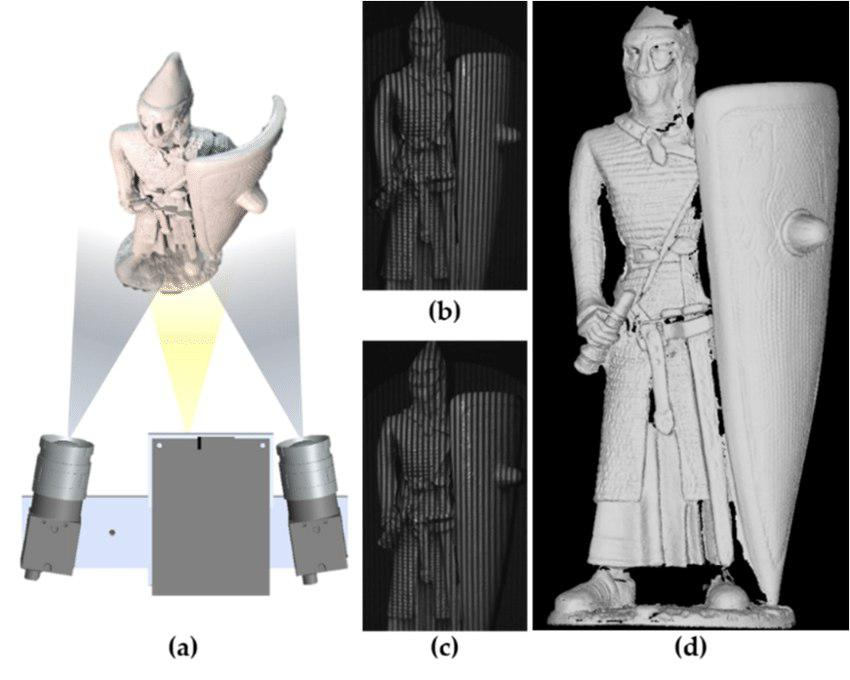
\includegraphics[scale=0.1]{pictures/polop5}
\end{figure}
\begin{itemize}
\item Mitigates multipath reflections
\item Improves robustness
\item Avoids interference between multiple systems
\item BUT correspondence search has high computational cost!
\end{itemize}

\end{frame}


%%%%%%%%%%%%%%%%%%%%%%%%%%%%%%%%%%%%%%%%%%%%%%%%%%%%%%%%%%%%%%%%%%%%%%%%%%%%%%%%%
%
% Jasi's part <3
%
%%%%%%%%%%%%%%%%%%%%%%%%%%%%%%%%%%%%%%%%%%%%%%%%%%%%%%%%%%%%%%%%%%%%%%%%%%%%%%%%%
\section{UltraStereoAlgorithm}
\subsection{}
\begin{frame}{UltraStereo}
\end{frame}

\begin{frame}{UltraStereo}
\begin{itemize}
\item two IR cameras: monochrome Ximea cameras, 1280x1024 pixel at 210Hz
\item DOE projector
\end{itemize}
\end{frame}

\begin{frame}

\begin{figure}
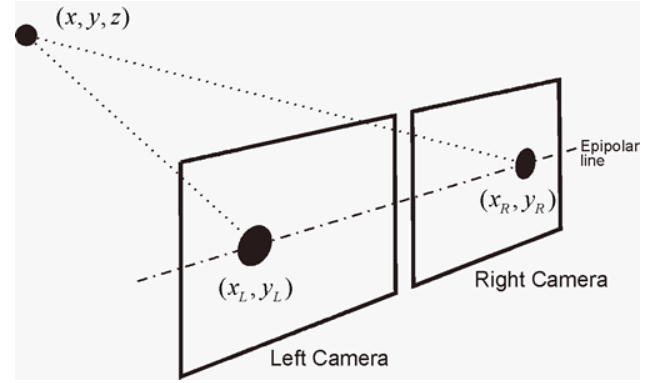
\includegraphics[scale=0.5]{pictures/disp}
\end{figure}
\begin{equation}
disparity = \frac{bf}{x_{L}- x_{R}}
\end{equation}
f = focal length\\
b = baseline
\end{frame}

\begin{frame}{Dimensionality Reduction}
\begin{figure}
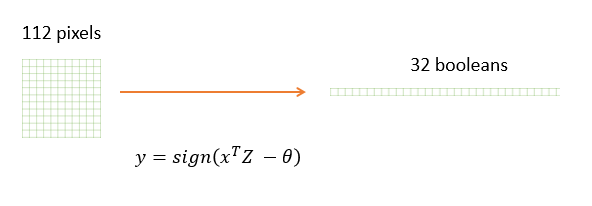
\includegraphics[scale=0.6]{pictures/patches}
\end{figure}
$ x \in R^{W} $  with W = 11x11\\
$ Z \in R^{b} $ with b = 32\\
$ \theta \in R^b$
$ y \in (0,1)^{b}
\end{frame}

\begin {frame}{How to chose the parameters}
\begin {figure}
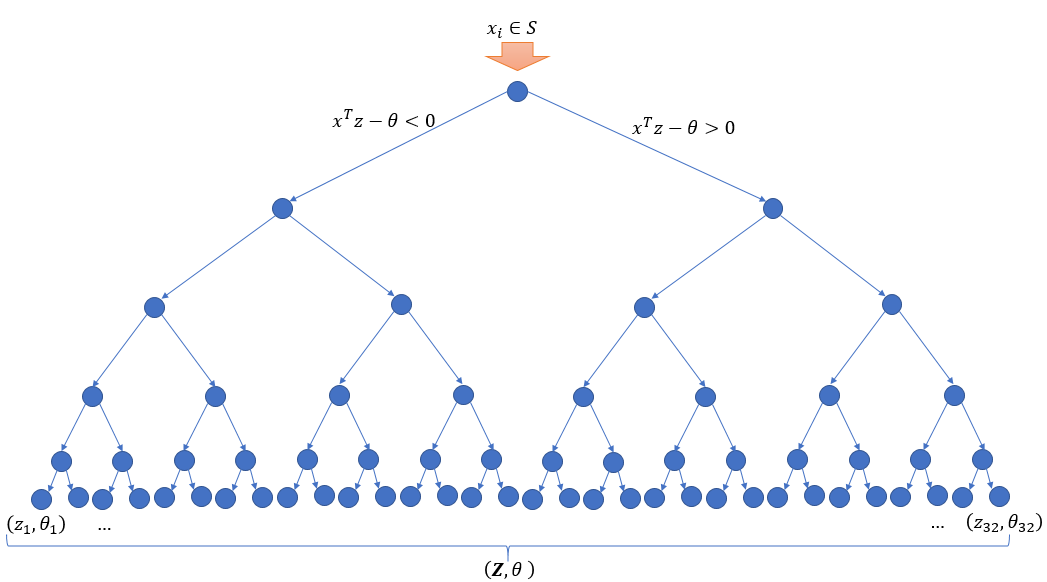
\includegraphics[scale=0.35]{pictures/tree}
\end {figure}

\begin{itemize}
\item k<< W -> sparse hyperplanes
\item Information gain: $I(\delta) = H(S) -\sum_{d\in L,R} \frac{S_{d}(\delta)}{S} H(S_{d}(\delta))$
\end{itemize}
$\delta$: set of learned parameters $(z,\theta)$
\end{frame}

%%%%%%%%%%%%%%%%%%%%%%%%%%%%%%%%%%%%%%%%%%%%%%%%%%%%%%%%%%%%%%%%%%%%%%%%%%%%%%%%%
%
% Julie's part
%
%%%%%%%%%%%%%%%%%%%%%%%%%%%%%%%%%%%%%%%%%%%%%%%%%%%%%%%%%%%%%%%%%%%%%%%%%%%%%%%%%
%\section{Test}
\subsection{Matching Framework}
\begin{frame}{Matching Framework}

\begin{itemize}
\item Based on PatchMatch framework
\item Iterative and randomized process
\item 3 steps: initialization, propagation, post-processing
\end{itemize}
\centering
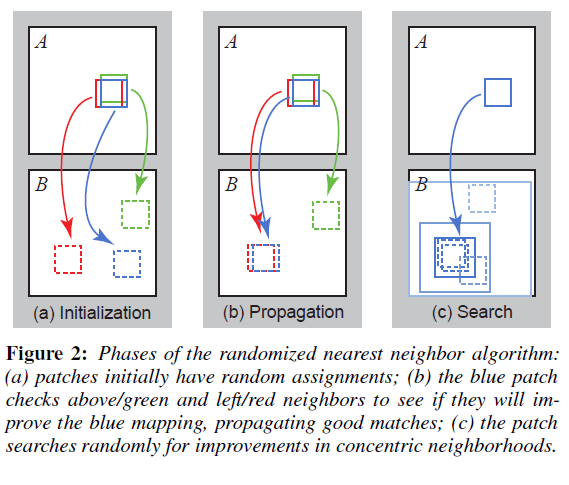
\includegraphics[scale=0.7]{pictures/fig1_patchmatch}
\end{frame}

\subsection{Computational Analysis}
\begin{frame}{Computational Analysis}
\begin{itemize}
\item Linear with respect to the image size
\item O(1) complexity of the binary representation
\end{itemize}
\end{frame}

\section{Evaluation}% To vanish after the other parts are done ! 
\subsection{Quantitative evaluation}
\begin{frame}{Quantitative evaluation}
\begin{itemize}
\item 2500 training images and 900 test images (500 articulated hand images and 400 interior images for 5 different environments)
\end{itemize}
\centering
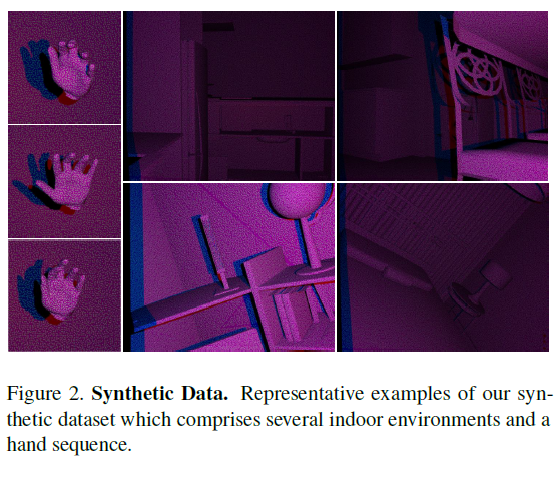
\includegraphics[scale=0.7]{pictures/fig2_synthetic_data}
\end{frame}

\subsection{Bias}
\begin{frame}{Bias}
\begin{itemize}
\item Average absolute depth error present in the whole set
\end{itemize}
\begin{figure}
\centering
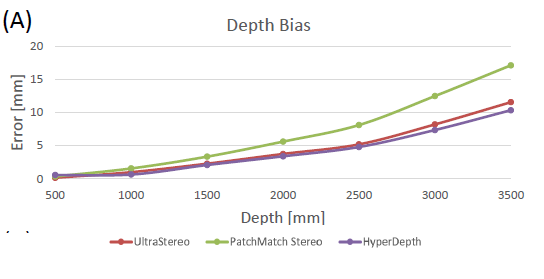
\includegraphics[scale=1]{pictures/fig3_depth_Bias_synthetic_data}
\caption{synthetic data}
\end{figure}
\end{frame}

\begin{frame}{Bias}
\begin{figure}
\centering
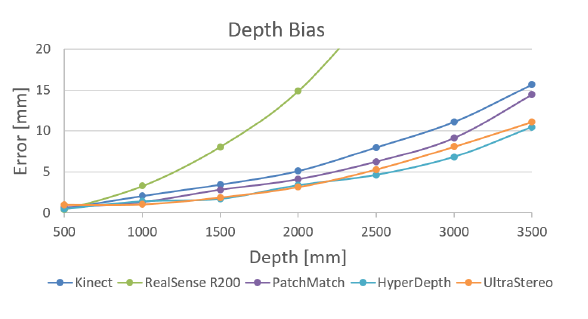
\includegraphics[scale=1]{pictures/fig_4_depth_bias_real_data}
\caption{real data}
\end{figure}
\end{frame}



%%%%%%%%%%%%%%%%%%%%%%%%%%%%%%%%%%%%%%%%%%%%%%%%%%%%%%%%%%%%%%%%%%%%%%%%%%%%%%%%%
%
% John's part
%
%%%%%%%%%%%%%%%%%%%%%%%%%%%%%%%%%%%%%%%%%%%%%%%%%%%%%%%%%%%%%%%%%%%%%%%%%%%%%%%%%
\section{LOL}% To vanish after the other parts are done ! 
\subsection{Invalidation}
\begin{frame}{Invalidation}
Issues which the pixels from the final depth image won't contain any estimations :
\begin{itemize}
\item Oculusions
\item Saturation of infrared sensors
\item low signal noise ratio
\end{itemize}
How limits this errors ?
\begin{itemize}
\item an algorithms does an invalidation pass durint the post-processing step
\end{itemize}
\end{frame}

\begin{frame}{Invalidation}
\begin{figure}
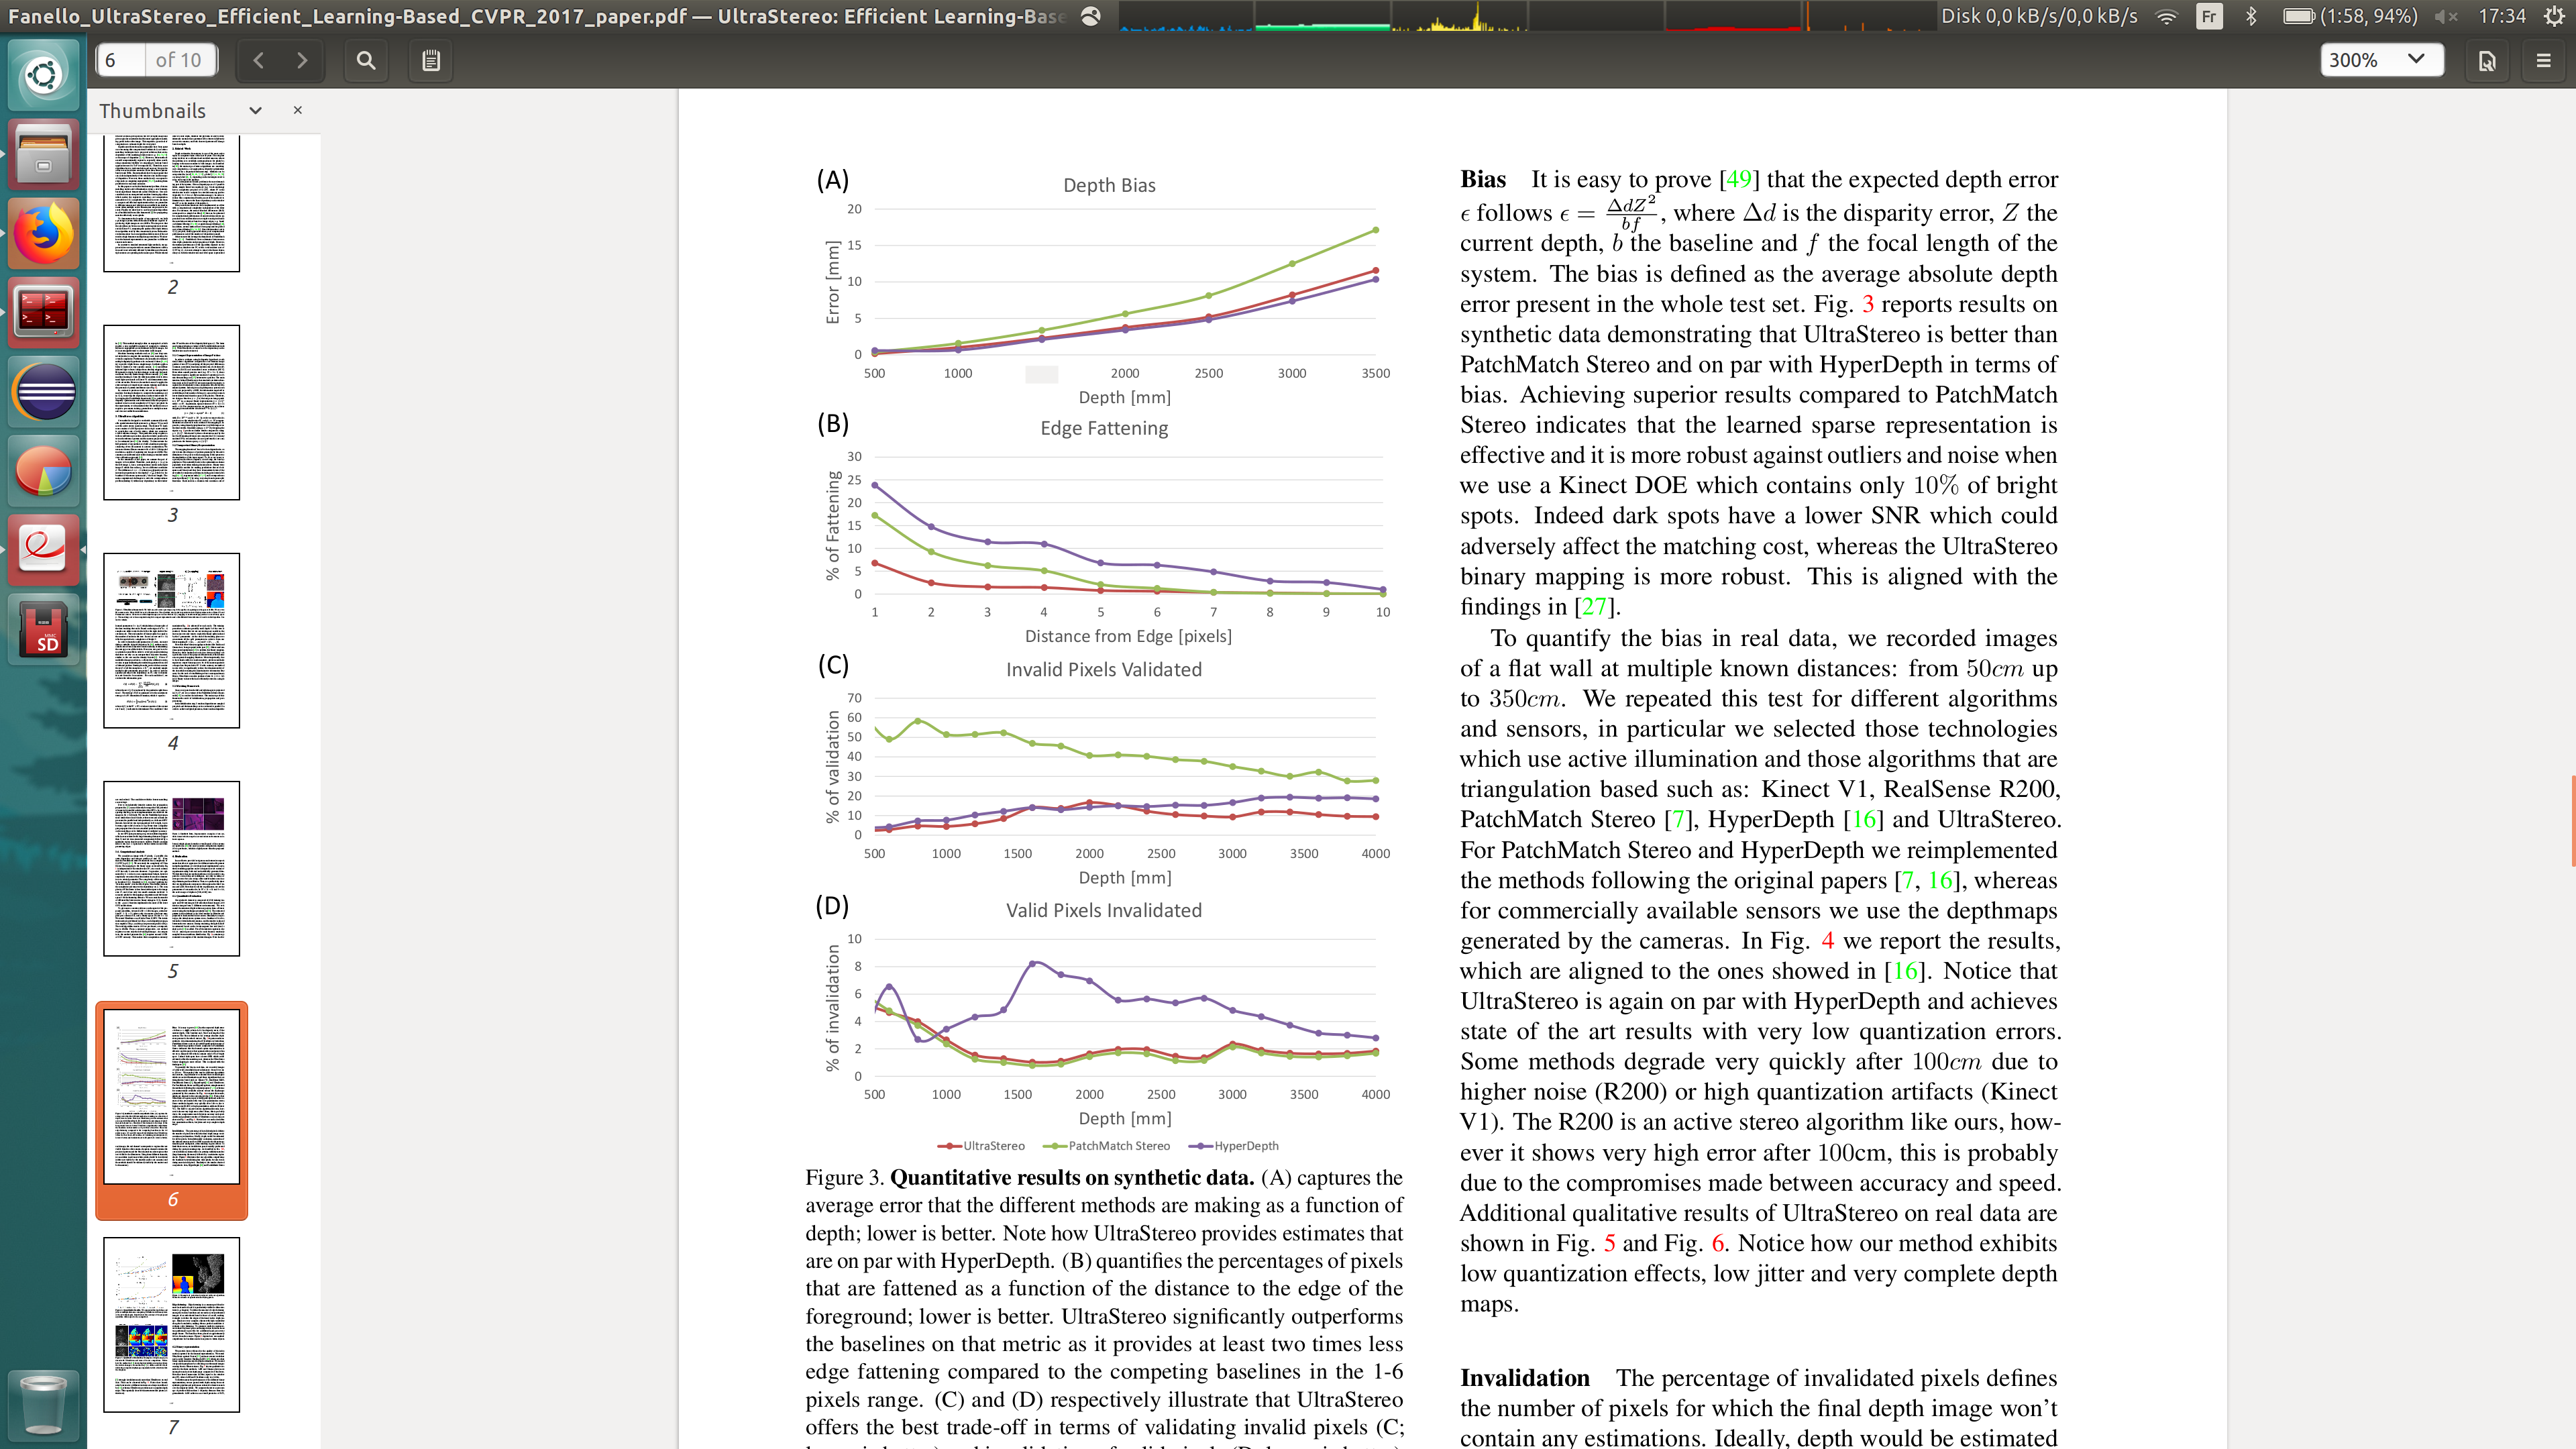
\includegraphics[scale=0.06]{pictures/fig3}
\caption{Quantitative results on syntatic data}
\end{figure}
\end{frame}

\begin{frame}{Example of depth-map produced with UltraStereo}
Look at the thin structures like plants
\begin{figure}
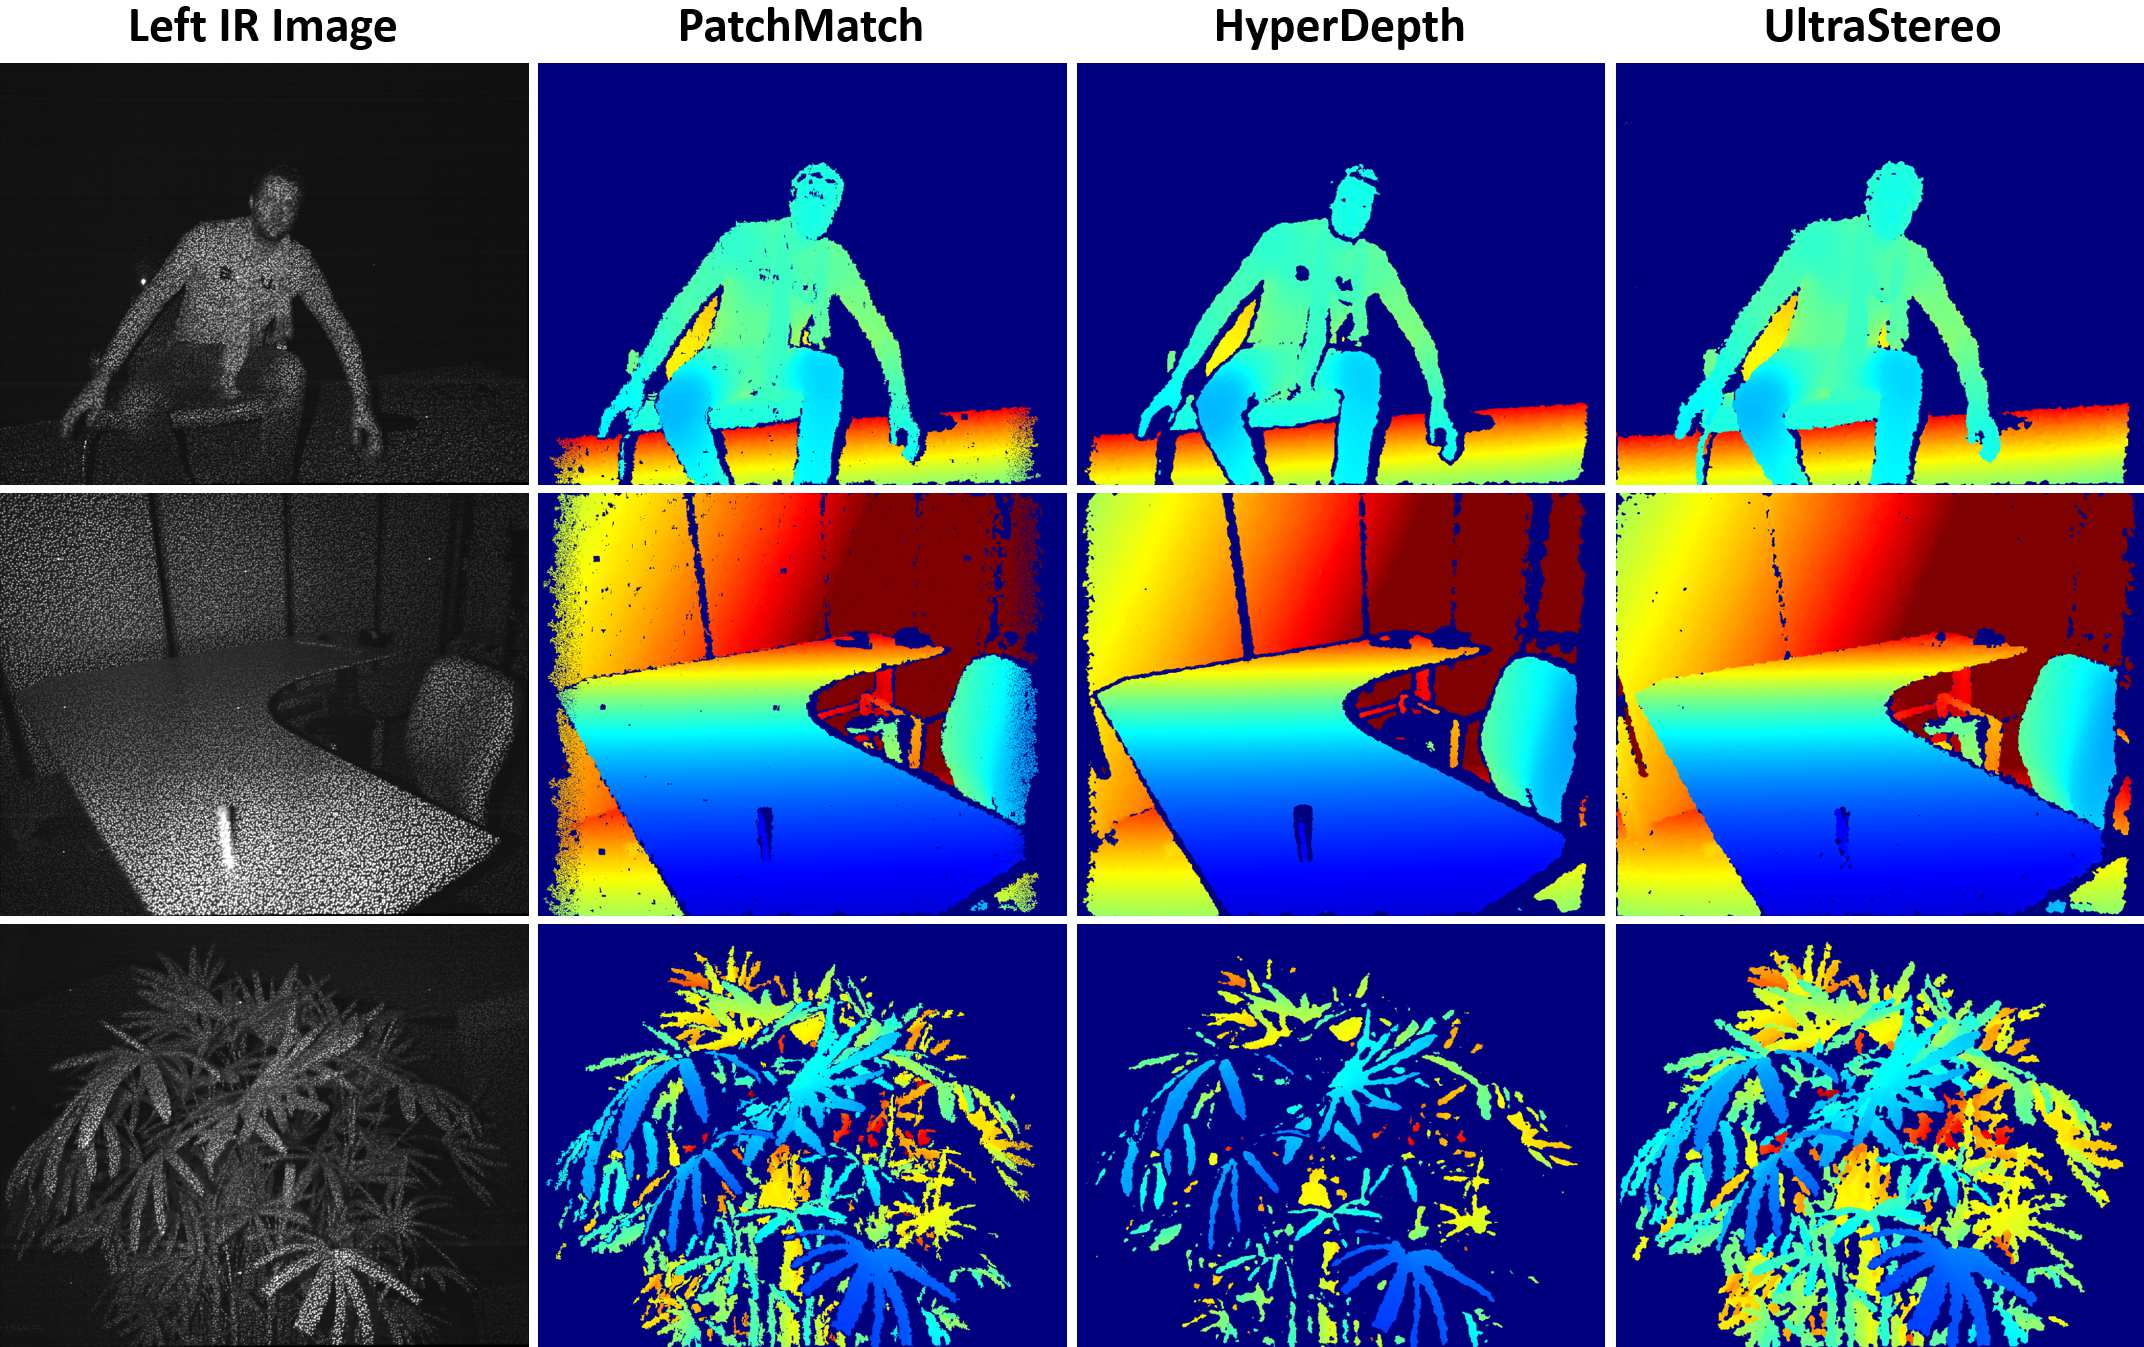
\includegraphics[scale=0.08]{pictures/fig5}
\caption{Qualitative Evaluation}
\end{figure}
\end{frame}

\begin{frame}{Edge fattening}
Other issiue is the edge fattening. To measure it they :
\begin{itemize}
\item used a hand to test their algorithms
\item put a hand at 1 m from the sensors
\item defined key hand pose for each frame
\end{itemize}
\end{frame}

\begin{frame}{Edge fattening}

\begin{figure}
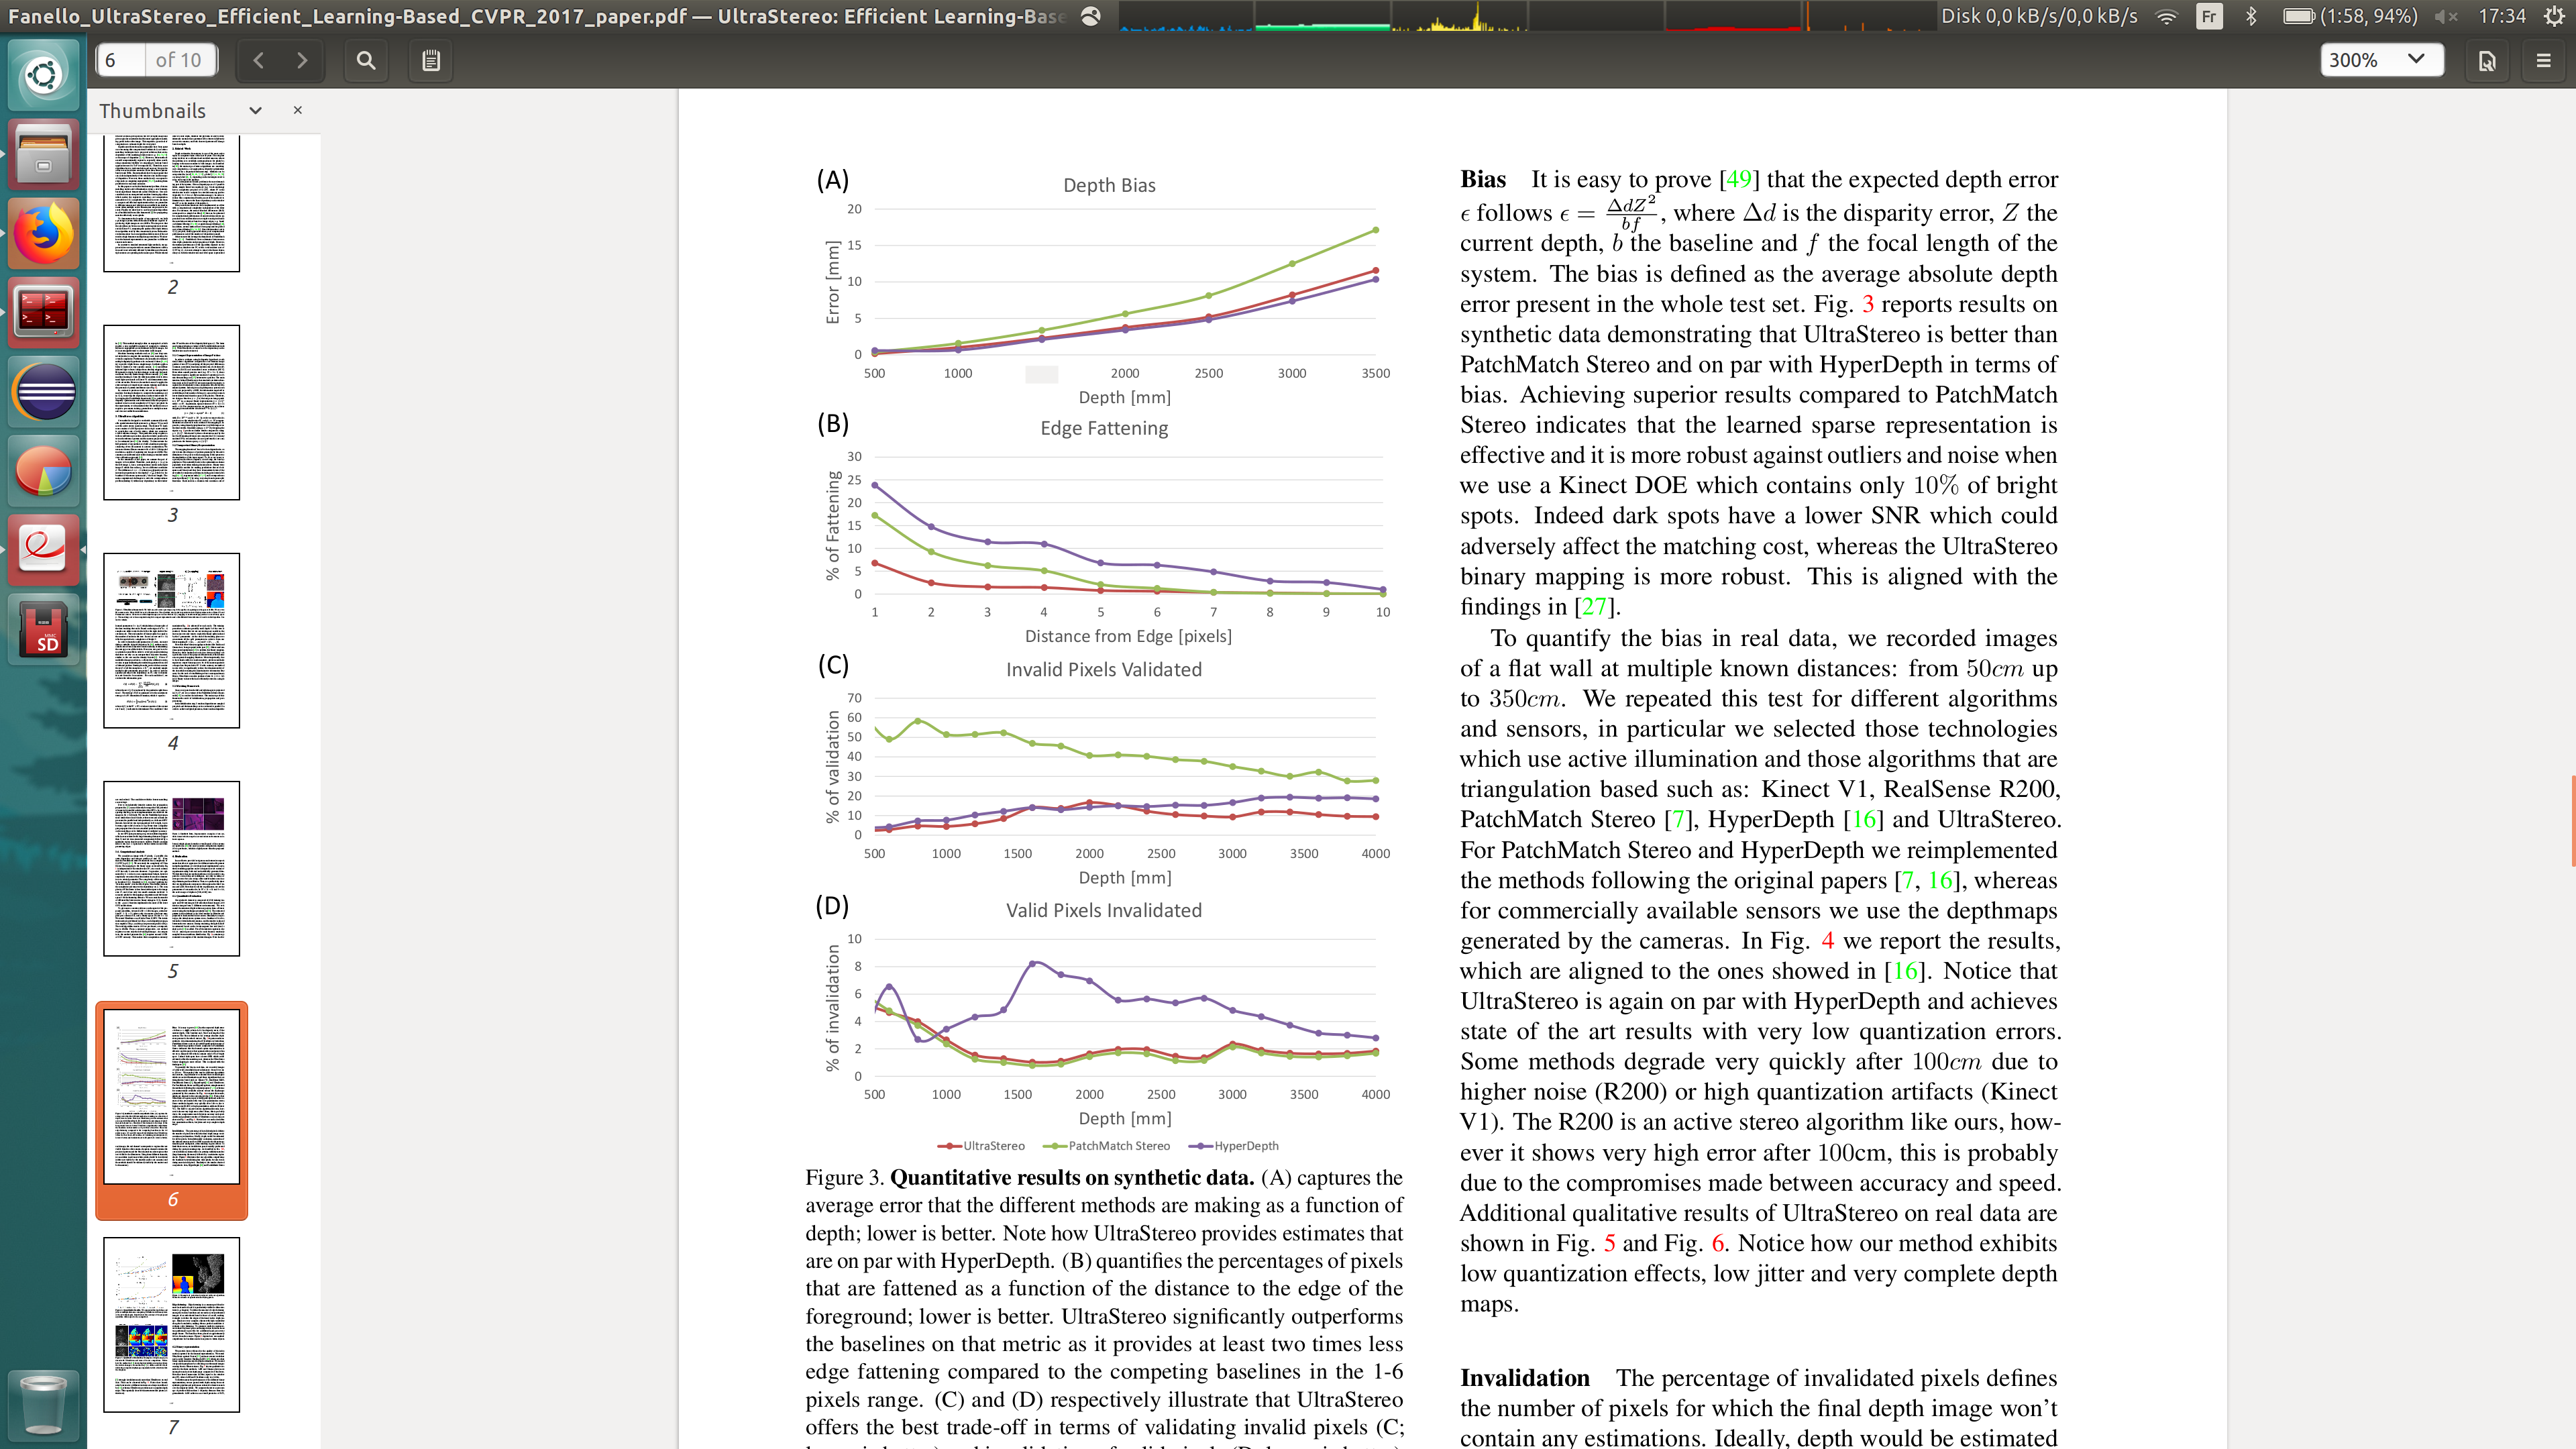
\includegraphics[scale=0.06]{pictures/fig3}
\caption{Quantitative results on syntatic data}
\end{figure}
\end{frame}

\begin{frame}{Edge fattening}

\begin{figure}
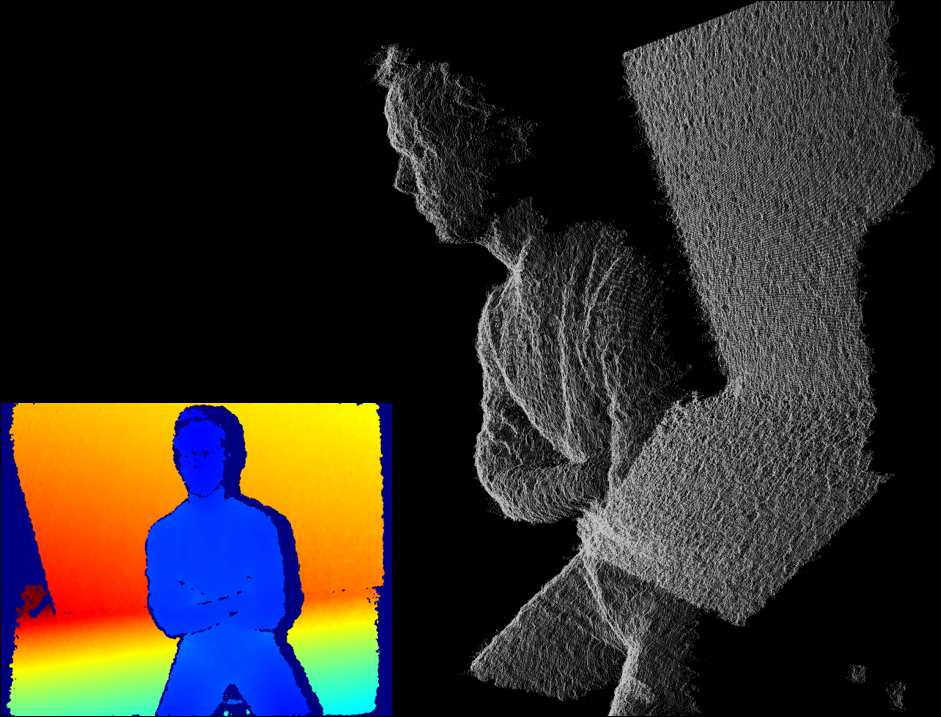
\includegraphics[scale=0.15]{pictures/fig6}
\caption{???}
\end{figure}
\end{frame}

\subsection{Binary representation}
\begin{frame}{Binary representation}
\begin{itemize}
\item Compare UltraStereo with Census and Locality Sensitive Hashing (LSH)
\item Collect 1000 images with the Kinnect
\end{itemize}
\begin{figure}
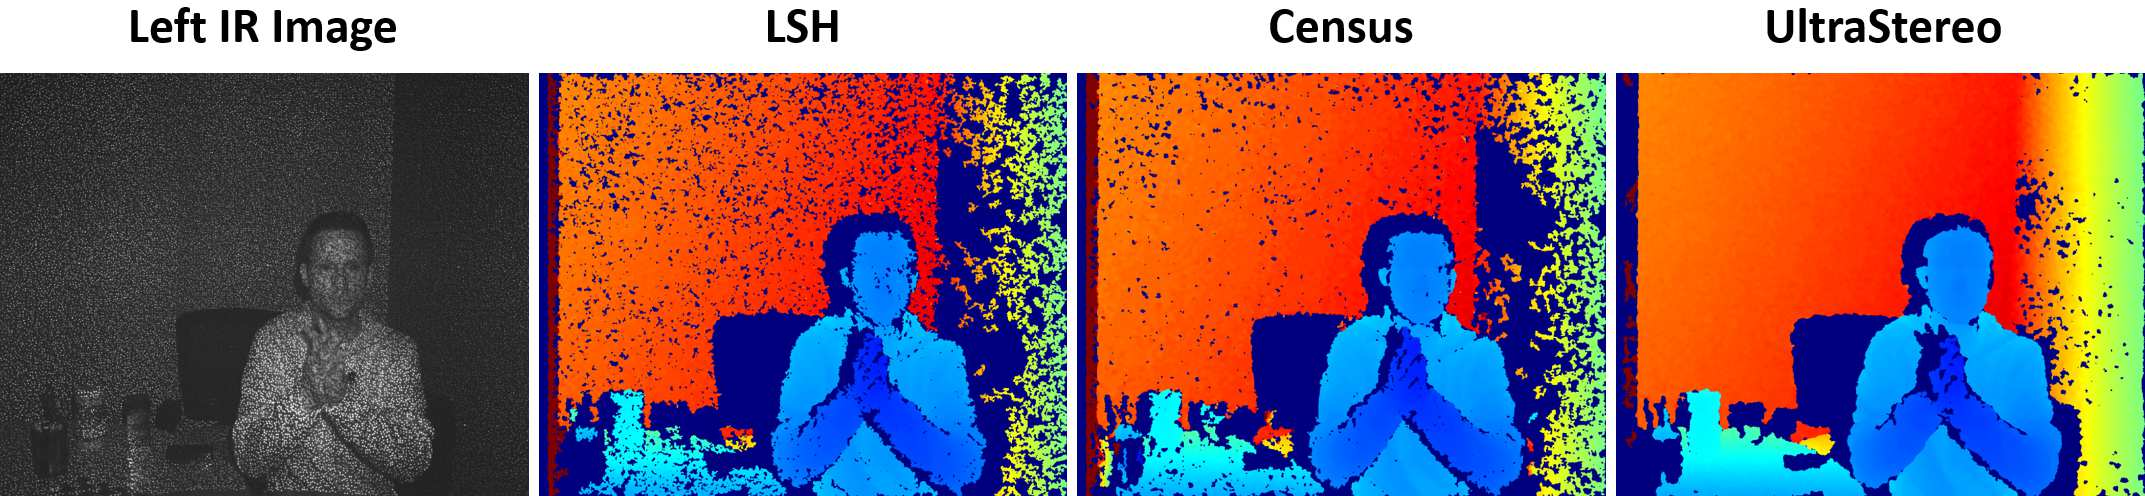
\includegraphics[scale=0.1]{pictures/fig7}
\caption{Census use 121 bits, LSH and UltraStereo use only 32 bits}
\end{figure}
\end{frame}

\subsection{Interference and Generalization}
\begin{frame}{Interferenc and Generalization}
\begin{figure}
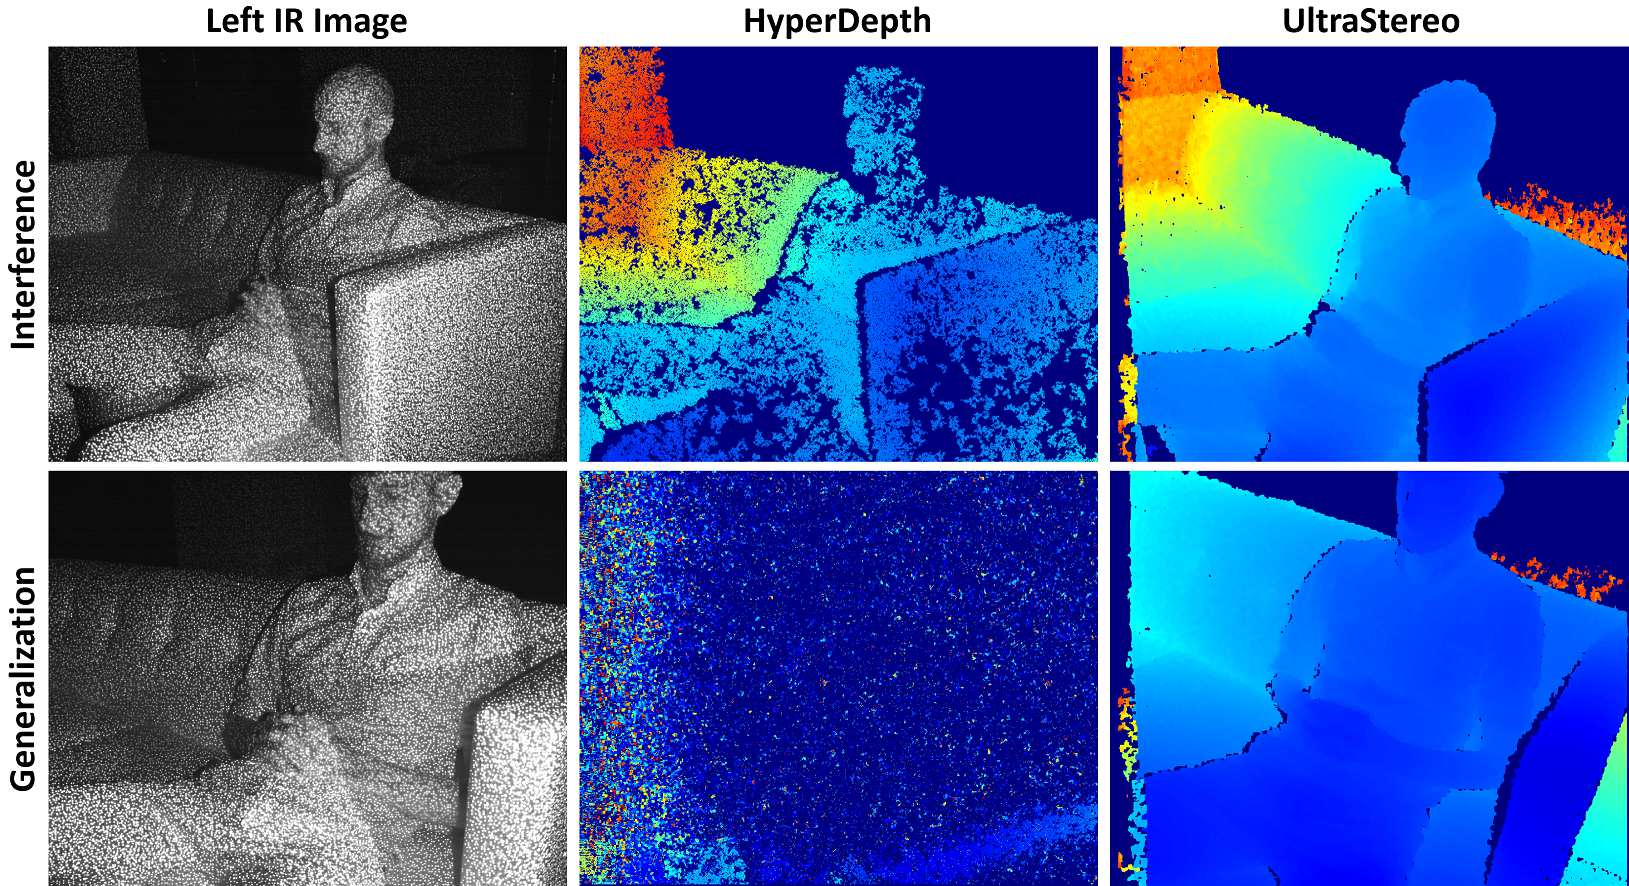
\includegraphics[scale=0.08]{pictures/fig8}
\caption{}
\end{figure}
\end{frame}

\section{Conclusion}
\begin{frame}{Conclusion}
Best algorithms ever made !
\end{frame}


%%%%%%%%%%%%%%%%%%%%%%%%%%%%%%%%%%%%%%%%%%%%%%%%%%%%%%%%%%%%%%%%%%%%%%%%%%%%
%
% Questions, etc...
%
%%%%%%%%%%%%%%%%%%%%%%%%%%%%%%%%%%%%%%%%%%%%%%%%%%%%%%%%%%%%%%%%%%%%%%%%%%%%
\section{Questions ?}
\begin{frame}{Questions}
\centering
\Huge{?}
\end{frame}

\begin{frame}{}
\centering
\Huge{Thank you for your attention !}
\end{frame}



\end{document}%Document end *************************************************
